\documentclass[12pt, a4paper]{article}

\usepackage{changepage,titlesec}

\titleformat{\section}[block]{\bfseries\LARGE}{\thesection.}{1em}{}
\titleformat{\subsection}[block]{\bfseries\normalsize}{\thesubsection}{1em}{}
\titleformat{\subsubsection}[block]{\bfseries\normalsize}{\thesubsubsection}{1em}{}
\titlespacing*{\subsection} {2em}{3.25ex plus 1ex minus .2ex}{1.5ex plus .2ex}
\titlespacing*{\subsubsection} {5em}{3.25ex plus 1ex minus .2ex}{1.5ex plus .2ex}

\usepackage[T1]{fontenc}
\usepackage{style}
\usepackage{tabularx}
\usepackage{ltablex}
\usepackage{graphicx}
\usepackage[colorlinks=true,linkcolor=blue]{hyperref}
\usepackage{float}
\usepackage{titlesec}

\setlength{\parindent}{0pt}

\newcommand{\sectionbreak}{\clearpage}

\pdfadjustspacing=4
\DeclareGraphicsExtensions{.pdf,.png,.jpg,.bmp}
\graphicspath{ {./diagramy/} }
\title{System zarządzania zasobami ludzkimi w firmie}
\author{Katarzyna Kucharczyk, Michał Mazek, Łukasz Żmuda, Michał Barański}

\begin{document}
   \maketitle
   \tableofcontents
	\section{Analiza wymagań}
System skierowany jest do firm zajmujących się wytwarzaniem produktów IT. Skierowany jest do wszystkich zatrudnionych w firmie, z głównym wskazaniem na:
\begin{itemize*}
\item menadżerów projektów,
\item pracowników technicznych (programistów, testerów)
\item analityków.
\end{itemize*}

System ma za zadanie wspomagać zarządzanie projektami pod kątem zasobów niezbędnych do ich wytwarzania. Ma umożliwiać stałe monitorowanie kosztów projektu i zapewniać możliwość szybkich reakcji w dynamicznie zmieniającym się środowisku.
\subsection{Wymagania funkcjonalne}
Głównym zadaniem systemu jest wsparcie zarządzania projektami pod kątem:

\begin{tabular}{|c|c|c|c|}
\hline 
Lp. & Nazwa & Opis & Priorytet \\ 
\hline 
F1 & Tworzenie zespołów & • & Wysoki \\ 
\hline 
F2 & Zarządzanie zespołami & • & Wysoki \\ 
\hline 
F3 & Dodwanie pracowników & • & Wysoki \\ 
\hline 
F3 & Zarządzanie/edycja profilów pracowników & Możliwość uzupełnienia profilu pracownika o dodatkowe doświadczenia & • \\ 
\hline 
F4 & Alokacja pracowników & Przypisywanie pracowników do zespołów projektowych & Wysoki \\ 
\hline 
F5 & Tworzenie harmonogramów & • & Wysoki \\ 
\hline 
F6 & Zarządzanie harmonogramami & • & Wysoki \\ 
\hline 
F7 & • & • & • \\ 
\hline 
F9 & • & • & • \\ 
\hline 
F10 & • & • & • \\ 
\hline 
F11 & • & • & • \\ 
\hline 
\end{tabular} 
\begin{enumerate}
\item planowania i śledzenia czasu pracy pracowników firmy,
\item definiowania i raportowania kosztów projektów,
\item zarządzania dostępnym czasem pracowników,
\item przechowywaniem profili pracowników i możliwość ich wygodnego przeglądania i przeszukiwania,
\item definiowania struktury firmy (menadżerowie i podwładni),
\item monitorowania postępów projektów.
\end{enumerate}

\subsection{Wymagania niefunkcjonalne}

\begin{tabular}{|c|c|c|c|}
\hline 
Lp. & Nazwa & Opis & Priorytet \\ 
\hline 
NF1 & • & • & • \\ 
\hline 
NF2 & • & • & • \\ 
\hline 
NF3 & • & • & • \\ 
\hline 
NF3 & • & • & • \\ 
\hline 
NF4 & • & • & • \\ 
\hline 
NF5 & • & • & • \\ 
\hline 
NF6 & • & • & • \\ 
\hline 
NF7 & • & • & • \\ 
\hline 
NF9 & • & • & • \\ 
\hline 
NF10 & • & • & • \\ 
\hline 
NF11 & • & • & • \\ 
\hline 
\end{tabular}

Aplikacja będzie używana przez różne osoby w firmie. W ramach aplikacji zdefiniowane są następujące role, jakie pełnione są przez użytkowników:
\begin{itemize*}
\item \textbf{Menadżer zespołu} - w ramach tej roli ...
\item Menadżer projektu
\item Pracownik HR
\item Pracownik techniczny
\end{itemize*}
W ramach każdej roli zdefiniowany jest inny zakres możliwości i funkcji dostępnych w systemie.


	\section{Przypadki użycia}
Wszelkie przypadki użycia posiadają warunek poprawnego przejścia scenariusza pierwszego (UC1 Autoryzacja użytkownika).
\begin{enumerate}
\item Autoryzacja użytkownika \\
Nazwa: UC1 Autoryzacja użytkownika \\
Opis: Proces logowania się pracownika \\
Aktorzy: Uzytkownik \\
Warunki początkowe: 
\begin{itemize}
\item Istniejące konto w systemie 
\end{itemize}
Warunki końcowe: 
\begin{itemize}
\item Dostęp do systemu 
\end{itemize}
Scenariusz główny:
\begin{enumerate}
\item Aktor wprowadza swoje login i hasło
\item System sprawdza zapytanie
\item System wyświetla ekran powitalny
\end{enumerate}
Scenariusz alternatywny - błędne dane: 
\begin{enumerate}
\item Aktor wprowadza swoje login i hasło
\item System uznaje zapytanie za błędne
\item System wyświetla ekran informujacy o błędnym loginie lub haśle
\end{enumerate}

\item Dodanie/edycja profilu użytkownika \\
Nazwa: UC2 Dodanie/edycja profilu użytkownika \\
Opis: Proces dodania/edycji profilu dla pracownika \\
Aktorzy: HR \\
Warunki początkowe:
\begin{itemize}
\item Dokument z informacjami dotyczącymi pracownika
\end{itemize}
Warunki końcowe: 
\begin{itemize}
\item Uaktualniony profil pracownika
\end{itemize}
Scenariusz główny:
\begin{enumerate}
\item Aktor otwiera formularz profilu pracownika
\item Aktor uzupełnia/zmienia wybrane pola
\item Aktor potwierdza zmiany odpowiednim przyciskiem
\item System zapisuje w bazie danych nowe dane
\item System wyświetla ekran poglądowy z nowym profilem użytkownika
\end{enumerate}
Scenariusz alternatywny - walidacja danych: 
\begin{enumerate}
\item Jak a-c jak w scenariuszu głównym
\item System wykrywa błędnie wpisane dane 
\item System zwraca formularz z zaznaczonymi błędnymi polami
\end{enumerate}
Scenariusz alternatywny - utrata łączności: 
\begin{enumerate}
\item Jak a-c jak w scenariuszu głównym
\item System ma problem z łącznością 
\item System wyświetla formularz, wraz z informacją o nie zapisaniu danych spowodowanych problemem łączności
\end{enumerate}
Scenariusz alternatywny - kolizja transakcji: 
\begin{enumerate}
\item Jak a-c jak w scenariuszu głównym
\item System wykrywa błąd transakcji (np. zakleszczenie)
\item System wyświetla formularz, wraz z prośbą o ponowienie zapytania
\end{enumerate}

\item Usuwanie profilu użytkownika \\
Nazwa: UC3 Usuwanie profilu użytkownika \\
Opis: Proces usuwania profilu dla pracownika \\
Aktorzy: HR lub Administrator \\
Warunki początkowe:
\begin{itemize}
\item Informacja o koncie do usunięcia
\end{itemize}
Warunki końcowe: 
\begin{itemize}
\item Zauktualizowana baza danych pozbawiona nieporządanego konta
\end{itemize}
Scenariusz główny:
\begin{enumerate}
\item Aktor otwiera listę użytkowników
\item Aktor wybiera opcje usunięcie konta przy nazwisku
\item System usuwa rekord z informacjami o użytkowniku
\item System wyświetla nową listę użytkowników
\end{enumerate}
Scenariusz alternatywny - błąd usuwania: 
\begin{enumerate}
\item Jak a-b jak w scenariuszu głównym
\item System wykrywa błęd podczas usuwania rekordu
\item System zwraca pierwotną listę z informacją z błędem usuwania
\end{enumerate}

\item Zmiana praw dostępu \\
Nazwa: UC4 Zmiana praw dostępu \\
Opis: Proces zmiany uprawnień użytkownika do określonych modułów. \\
Aktorzy: Administrator \\
Warunki początkowe:
\begin{itemize}
\item Dotychczas nadane prawa 
\end{itemize}
Warunki końcowe: 
\begin{itemize}
\item Uaktualniony profil z nowymi rolami
\end{itemize}
Scenariusz główny: 
\begin{enumerate}
\item Aktor wybiera z listy edytowane konto użytkownika
\item System wyświetla detale profilu użytkownika
\item Aktor wybiera odpowiednią opcję ról i zatwierdza
\item System zmienia rekord dotyczący ról dla danego konta
\item System zwraca widok profilu użytkowanika z nowymi prawami dostępu
\end{enumerate}
Scenariusz alternatywny - błąd zmiany : 
\begin{enumerate}
\item Jak a-c jak w scenariuszu głównym
\item System wykrywa kolizję lub bład połączenia
\item System wyświetla detale profilu użytkownika wraz z kodem błędu, który wystąpił
\end{enumerate}

\item Edycja zwierzchnictwa \\
Nazwa: UC5 Edycja zwierzchnictwa \\
Opis: Proces zmiany hierarchii drzewa struktury firmy. \\
Aktorzy: Administrator, HR lub kierownik projektu \\
Warunki początkowe:
\begin{itemize}
\item Dokument dotyczący hierarchii firmy
\end{itemize}
Warunki końcowe:
\begin{itemize}
\item Uaktualnione drzewo hierarchii w systemie 
\end{itemize}
Scenariusz główny:
\begin{enumerate}
\item Aktor wybiera z listy edytowane konto użytkownika
\item System wyświetla detale profilu użytkownika
\item Aktor wybiera użytkownika który ma być zwierzchnikiem dla edytowanego użytkownika
\item System zmienia rekord dotyczący zwierzchnika
\item System zwraca nowy widok profilu użytkowanika
\end{enumerate}
Scenariusz alternatywny - wykrycie pętli: 
\begin{enumerate}
\item Jak a-c jak w scenariuszu głównym
\item System wykrywa pętle w drzewie hierarchii
\item System wyświetla informacje o błędzie
\end{enumerate}

\item Tworzenie projektu \\
Nazwa: UC6 Tworzenie projektu\\
Opis: Proces odpowiedzialny za tworzenie projektu\\
Aktorzy: Kierownik projektu \\
Warunki początkowe:
\begin{itemize}
\item Brak projektu w systemie.
\end{itemize}
Warunki końcowe:
\begin{itemize}
\item Nowy projekt w systemie, bez stworzonych zadań.
\end{itemize}
Scenariusz główny:
\begin{enumerate}
\item Aktor wybiera utworzenie nowego projektu.
\item System wyświetla formularz z pustymi polami (Nazwa projektu, opis, data początkowa, data końcowa, status)
\item Aktor uzupełnia puste pola i zatwierdza.
\item System zwraca nowy widok z projektami, gdzie pojawia się nowo dodany projekt.
\end{enumerate}
Scenariusz alternatywny - podanie błędnych danych projektu: 
\begin{enumerate}
\item Jak a-c jak w scenariuszu głównym
\item System wyświetla informacje o błędzie
\item Aktor wprowadza prawidłowe dane
\item Jak d w scenariuszu głównym
\end{enumerate}

\item Modyfikacja projektu \\
Nazwa: UC7 Modyfikacja projektu\\
Opis: Proces odpowiedzialny za modyfikację projektu\\
Aktorzy: Kierownik projektu \\
Warunki początkowe:
\begin{itemize}
\item W systemie istnieje projekt.
\end{itemize}
Warunki końcowe:
\begin{itemize}
\item Zmodyfikowany projekt w systemie.
\end{itemize}
Scenariusz główny:
\begin{enumerate}
\item Aktor wybiera modyfikację projektu.
\item System wyświetla formularz z danymi projektu
\item Aktor zmienia pola i zatwierdza.
\item System zwraca nowy widok z projektami.
\end{enumerate}
Scenariusz alternatywny - podanie błędnych danych modyfikowanego projektu: 
\begin{enumerate}
\item Jak a-c jak w scenariuszu głównym
\item System wyświetla informacje o błędzie
\item Aktor wprowadza prawidłowe dane
\item Jak d w scenariuszu głównym
\end{enumerate}


\item Usunięcie projektu \\
Nazwa: UC8 Usunięcie projektu\\
Opis: Proces odpowiedzialny za usunięcie projektu\\
Aktorzy: Kierownik projektu \\
Warunki początkowe:
\begin{itemize}
\item W systemie istnieje projekt.
\end{itemize}
Warunki końcowe:
\begin{itemize}
\item W systemie nie ma projektu.
\end{itemize}
Scenariusz główny:
\begin{enumerate}
\item Aktor wybiera usunięcie projektu.
\item System wyświetla komunikat w celu potwierdzenia usunięcia.
\item Aktor zatwierdza wybór.
\item System zwraca widok z projektami.
\end{enumerate}
Scenariusz alternatywny - brak potwierdzenia: 
\begin{enumerate}
\item Jak a-b jak w scenariuszu głównym
\item Aktor nie potwierdza usunięcia.
\item Jak d w scenariuszu głównym
\end{enumerate}


\item Tworzenie zadania \\
Nazwa: UC9 Tworzenie zadania\\
Opis: Proces odpowiedzialny za tworzenie zadania\\
Aktorzy: Kierownik projektu, bądź pracownik techniczny \\
Warunki początkowe:
\begin{itemize}
\item W systemie nie ma informacji o zadaniu, należącym do projektu.
\end{itemize}
Warunki końcowe:
\begin{itemize}
\item Nowy utworzone zadanie należące do projektu.
\end{itemize}
Scenariusz główny:
\begin{enumerate}
\item Aktor wybiera interesujący go projekt.
\item System wyświetla listę zadań należących do projektu.
\item Aktor wybiera utworzenie nowego zadania.
\item System wyświetla formularz z pustymi polami (Nazwa zadania,opis, data początkowa, data końcowa, szacowane koszty, status)
\item Aktor uzupełnia puste pola i zatwierdza.
\item System zwraca nowy widok z projektem w którym pojawia się nowo utworzone zadanie.
\end{enumerate}
Scenariusz alternatywny - podanie błędnych danych zadania: 
\begin{enumerate}
\item Jak a-e jak w scenariuszu głównym
\item System wyświetla informacje o błędzie
\item Aktor wprowadza prawidłowe dane
\item Jak f w scenariuszu głównym
\end{enumerate}

\item Modyfikacja zadania \\
Nazwa: UC10 Modyfikacja zadania\\
Opis: Proces odpowiedzialny za modyfikację zadania\\
Aktorzy: Kierownik projektu, bądź pracownik techniczny \\
Warunki początkowe:
\begin{itemize}
\item W systemie istnieje zadanie nalezące do projektu.
\end{itemize}
Warunki końcowe:
\begin{itemize}
\item W systemie istnieje zmienione zadanie nalezące do projektu.
\end{itemize}
Scenariusz główny:
\begin{enumerate}
\item Aktor wybiera interesujący go projekt.
\item System wyświetla listę zadań należących do projektu.
\item Aktor wybiera modyfikację zadania.
\item System wyświetla formularz z danymi zadania.
\item Aktor zmienia dane i zatwierdza.
\item System zwraca nowy widok z projektem w którym pojawia się zmodyfikowane zadanie.
\end{enumerate}
Scenariusz alternatywny - podanie błędnych danych zadania modyfikowanego: 
\begin{enumerate}
\item Jak a-e jak w scenariuszu głównym
\item System wyświetla informacje o błędzie
\item Aktor wprowadza prawidłowe dane
\item Jak f w scenariuszu głównym
\end{enumerate}

\item Usunięcie zadania \\
Nazwa: UC11 Usunięcie zadania\\
Opis: Proces odpowiedzialny za usunięcie zadania\\
Aktorzy: Kierownik projektu, bądź pracownik techniczny \\
Warunki początkowe:
\begin{itemize}
\item W systemie istnieje zadanie nalezące do projektu.
\end{itemize}
Warunki końcowe:
\begin{itemize}
\item Brak zadania w systemie.
\end{itemize}
Scenariusz główny:
\begin{enumerate}
\item Aktor wybiera interesujący go projekt.
\item System wyświetla listę zadań należących do projektu.
\item Aktor wybiera usunięcie zadania.
\item System wyświetla komunikat w celu potwierdzenia usunięcia.
\item Aktor zatwierdza wybór.
\item System zwraca widok projektu bez usuniętego zadania.
\end{enumerate}
Scenariusz alternatywny - brak potwierdzenia usunięcia zadania: 
\begin{enumerate}
\item Jak a-d jak w scenariuszu głównym
\item Aktor nie zatwierdza wyboru.
\item System zwraca poprzedni widok projektu.
\end{enumerate}

\item Logowanie czasu pracy \\
Nazwa: UC12 Logowanie czasu pracy\\
Opis: Proces zalogowania informacji o tym, czym zajmował się pracownik, kiedy to robił i ile czasu na to poświęcił \\
Aktorzy: Pracownik techniczny \\
Warunki początkowe:
\begin{itemize}
\item Brak zalogowanych informacji z danego dnia, w zadaniu mogą istnieć logi z innych dat, bądź innych użytkowników.
\end{itemize}
Warunki końcowe:
\begin{itemize}
\item Zalogowane w odpowiednim zadaniu informacje.
\end{itemize}
Scenariusz główny:
\begin{enumerate}
\item Aktor wybiera projekt.
\item System wyświetla listę zadań należących do projektu.
\item Aktor wybiera zadanie do którego chce dodać loga.
\item System wyświetla listę logów należących do zadania.
\item Aktor wybiera dodanie nowego loga.
\item System wyświetla formularz z pustymi polami (czas pracy, opis, data początkowa, data końcowa)
\item Aktor uzupełnia puste pola i zatwierdza.
\item System zwraca nowy widok gdzie pojawia się nowo wprowadzony log z widoczną nazwą użytkownika, którego dotyczy.
\end{enumerate}
Scenariusz alternatywny - podanie błędnych danych w logu: 
\begin{enumerate}
\item Jak a-g jak w scenariuszu głównym
\item System wyświetla informacje o błędzie
\item Aktor wprowadza prawidłowe dane
\item Jak h w scenariuszu głównym
\end{enumerate}

\item Modyfikacja loga z czasem pracy \\
Nazwa: UC13 Modyfikacja loga z czasem pracy \\
Opis: Proces modyfikacji logowania.\\
Aktorzy: Pracownik techniczny \\
Warunki początkowe:
\begin{itemize}
\item Istnieje log w systemie.
\end{itemize}
Warunki końcowe:
\begin{itemize}
\item W systemie istnije zmodyfikowany log.
\end{itemize}
Scenariusz główny:
\begin{enumerate}
\item Aktor wybiera projekt.
\item System wyświetla listę zadań należących do projektu.
\item Aktor wybiera zadanie.
\item System wyświetla listę logów należących do zadania.
\item Aktor wybiera modyfikację loga.
\item System wyświetla formularz z treścią loga.
\item Aktor zmienia pola i zatwierdza.
\item System zwraca nowy widok gdzie pojawia się zmodyfikowany log z widoczną nazwą użytkownika, którego dotyczy.
\end{enumerate}
Scenariusz alternatywny - podanie błędnych danych w logu: 
\begin{enumerate}
\item Jak a-g jak w scenariuszu głównym
\item System wyświetla informacje o błędzie
\item Aktor wprowadza prawidłowe dane
\item System zwraca poprzedni widok zadania.
\end{enumerate}

\item Usunięcie loga z czasem pracy \\
Nazwa: UC14 Usunięcie loga z czasem pracy \\
Opis: Proces usunięcia loga z czasem pracy \\
Aktorzy: Pracownik techniczny \\
Warunki początkowe:
\begin{itemize}
\item W systemie istnieje log z czasem pracy.
\end{itemize}
Warunki końcowe:
\begin{itemize}
\item W systemie nie istnieje log z czasem pracy.
\end{itemize}
Scenariusz główny:
\begin{enumerate}
\item Aktor wybiera projekt.
\item System wyświetla listę zadań należących do projektu.
\item Aktor wybiera zadanie.
\item System wyświetla listę logów należących do zadania.
\item Aktor wybiera usunięcie loga.
\item System wyświetla komunikat w celu potwierdzenia usunięcia.
\item Aktor zatwierdza wybór.
\item System zwraca widok zadania bez usuniętego loga.
\end{enumerate}
Scenariusz alternatywny - brak potwierdzenia usunięcia loga: 
\begin{enumerate}
\item Jak a-d jak w scenariuszu głównym
\item Aktor nie zatwierdza wyboru.
\item System zwraca poprzedni widok zadania.
\end{enumerate}

\end{enumerate}
	\section{Architektura sytemu}
 
 
\subsection{Diagram komponentów}
Diagram komponentów przedstawia podział całego systemu na mniejsze podsystemy. Komponent jest to wymienny,wykonywalny fragment systemu. Zależności między komponentami są przedstawiane w postaci interfejsów tzn. jeden komponent może korzystać z funkcji jakie udostępnia inny komponent. Na rysunku \ref{fig:diagram_komponentow} przedstawiony jest diagram komponentów projektowanego systemu

\begin{figure}[h]
    \centering
    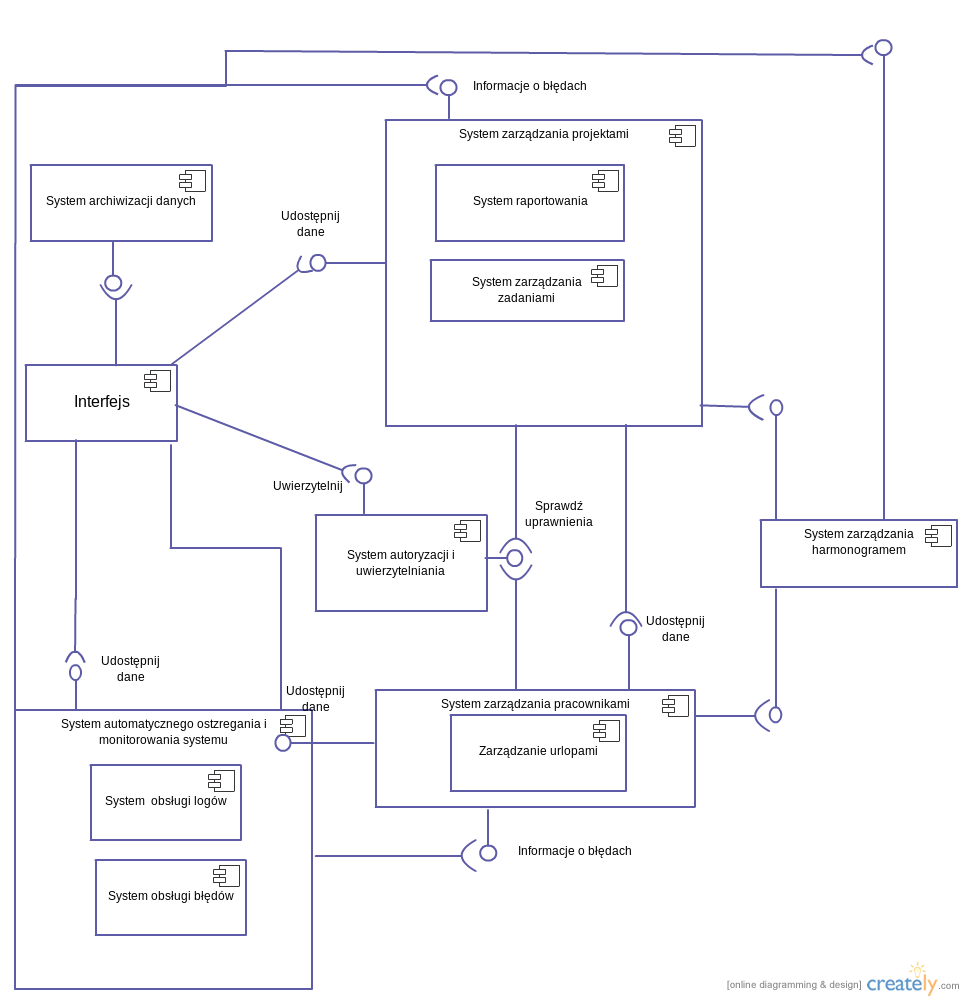
\includegraphics[scale=0.4]{diagramy/sekwencji_i_komponentow/diagram_komponentow.png}
    \caption{Diagram komponentów}
    \label{fig:diagram_komponentow}
\end{figure} 

Diagram na rysunku \ref{fig:diagram_komponentow} nie pokazuje pełnej struktury wewnętrznej wyszczególnionych podsystemów. Pokazanie zostały tylko najważniejsze komponenty tak aby rysunek pozostał czytelny. Na drugim diagramie komponentów \ref{fig:diag_kom_dane_dostep} przedstawiono w sposób bardzie szczegółowy to, że pod-systemy które korzystają z bazy danych zawierają w sobie komponenty (modele) których zadaniem jest komunikacja z bazą danych. Taka budowa systemów wynika z architektury MVC.

\begin{figure}[h]
    \centering
    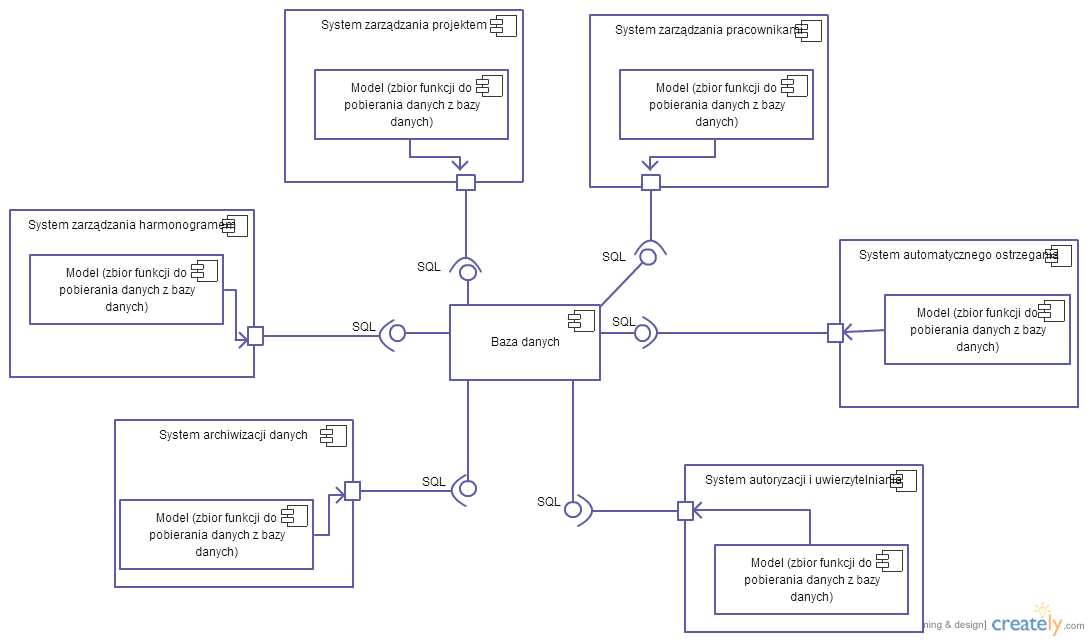
\includegraphics[scale=0.4]{diagramy/sekwencji_i_komponentow/diag_kom_dane_dostep.png}
    \caption{Diagram komponentów: dostęp do bazy danych}
    \label{fig:diag_kom_dane_dostep}
\end{figure} 
\subsection{Diagramy sekwencji}
W tym podrozdziale przedstawiono wybrane diagramy sekwencji. Diagram sekwencji obrazuje interakcje pomiędzy częściami systemu w postaci sekwencji komunikatów np. wywołań funkcji wymienianych między nimi. 

\begin{figure}[h]
    \centering
    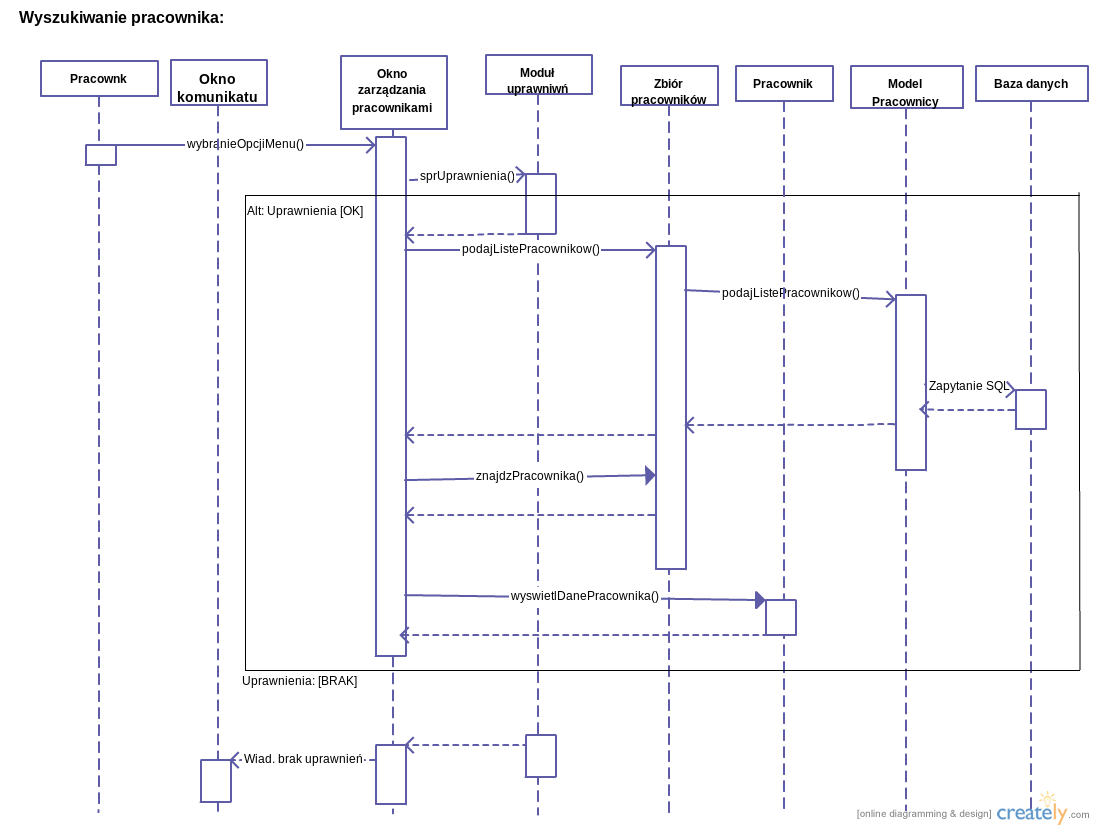
\includegraphics[scale=0.5, , angle=90 ]{./diagramy/sekwencji_i_komponentow/wyszukiwanie_pracownika.png}
    \caption{Diagram sekwencji: Wyszukiwanie pracownika}
    \label{fig:wyszukiwanie_pracownika}
\end{figure} 

\begin{figure}[h]
    \centering
    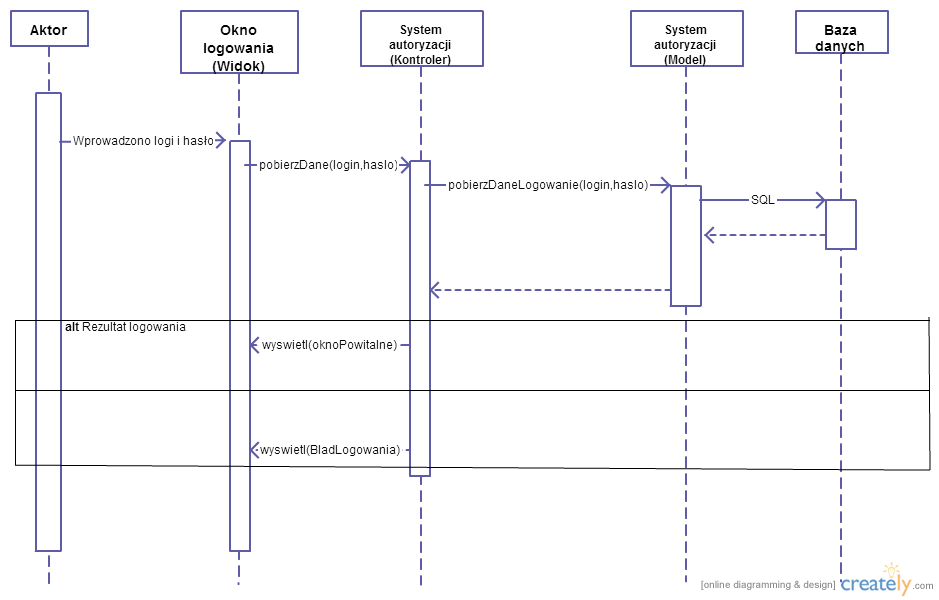
\includegraphics[scale=0.5]{./diagramy/sekwencji_i_komponentow/diag_sekwencji_logowanie.png}
    \caption{Diagram sekwencji: Logowanie do systemu}
    \label{fig:diag_sekwencji_logowanie.png}
\end{figure} 

section(Wymagania techniczne)
subsection{Wstępna specyfikacja sprzętu i oprogramowania podstawowego}
\begin{enumerate}
	\item System w wersji podstawowej będzie składał się z 2 serwerów. Każdy z serwerów będzie posiadał zainstalowany system Linux.
	\begin{itemize}
		\item serwer przechowywujący backendową część aplikacji, serwer webowy udostępniający usługę, oraz aplikację frontendową
		\item serwer przechowywujący bazę danych
	\end{itemize}
	
	\item Ze strony klienckiej wykorzystywana jest jedynie przeglądarka
	\item Komunikacja między serwerami oraz urządzeniami klientów jest zapewniona przez rounter sieci lokalnej z brakiem możliwości dostępu z zewnętrznej sieci
	\item Opcjonalnie możliwe jest użycie aplikacji przez skorzystanie z uslugi VPN uruchomionej na dodatkowym serwerze dostępowym
\end{enumerate}

\subsection{Specyfikacja technologii realizacji oprogramowania systemu}
\begin{enumerate}
	\item Aplikacja zostanie zrealizowana za pomocą technologii Java EE
	\item System bazy danych będzie zrealizowany jako baza NoSQL - w implementacji dokumentowej bazy danych MangoDB. Rozwiązanie to umżliwia szybki dostęp do ustrukturyzowanych danych.
	\item Aplikacja kliencka musi działać i być wyświetlana poprawnie pod przeglądarkami Chrome, Opera i Firefox, oraz Internet Explorer w wersji 8 i wyżej
	\item Frontend aplikacji klienckiej zostanie zrealizowany w technologii HTML5, CSS 3.00 oraz JavaScript
Jako serwer webowy zostanie użyty GlassFish Server

	\section{Diagramy przypadków użycia}

\subsection{Ekran logowania do systemu}
\begin{figure}[H]
    \centering
    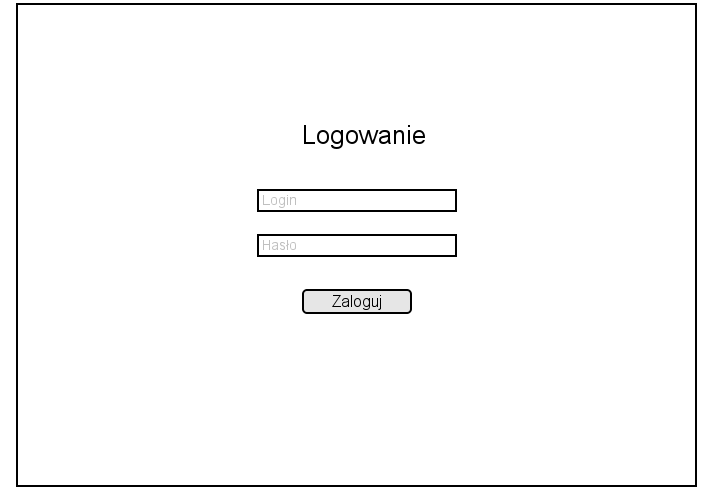
\includegraphics[scale=0.7]{diagramy/intefejsy/Logowanie.png}
    \caption{Logowanie}
    \label{fig:usecase}
\end{figure}

\subsection{Ekran logowania do systemu}
\begin{figure}[H]
    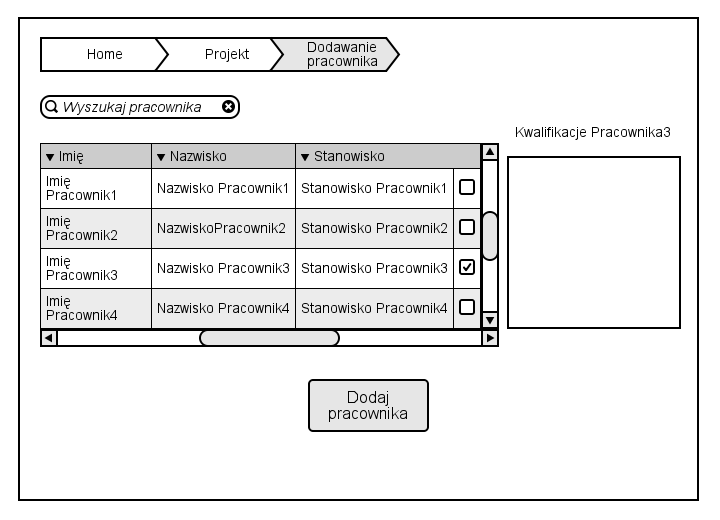
\includegraphics[scale=0.7]{diagramy/intefejsy/Dodanie_pracownika_do_projektu.png}
    \caption{Dodanie pracownika do projektu}
    \label{fig:usecase}
\end{figure}

\subsection{Ekran generowania raportu wedłóg użytkownika}
\begin{figure}[H]
    \centering
    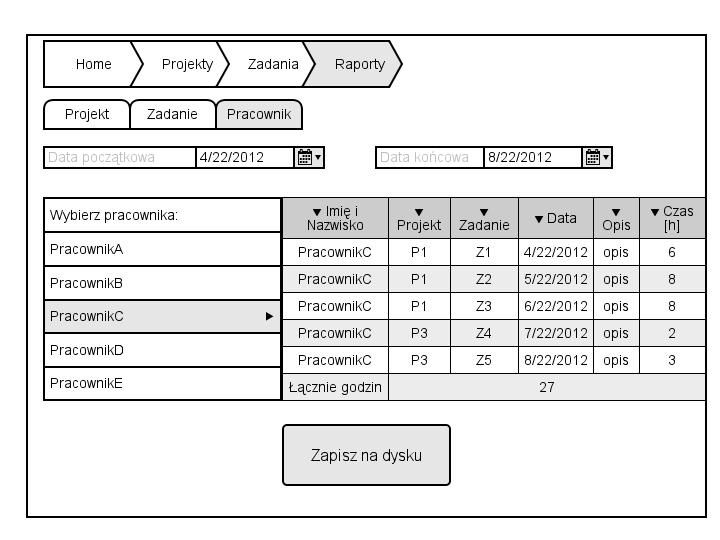
\includegraphics[scale=0.7]{diagramy/intefejsy/Generowanie_raportu_dla_uzytkownika.png}
    \caption{Generowanie raportu dla uzytkownika}
    \label{fig:usecase}
\end{figure}

\subsection{Ekran generowania raportu wedłóg zadania}
\begin{figure}[H]
    \centering
    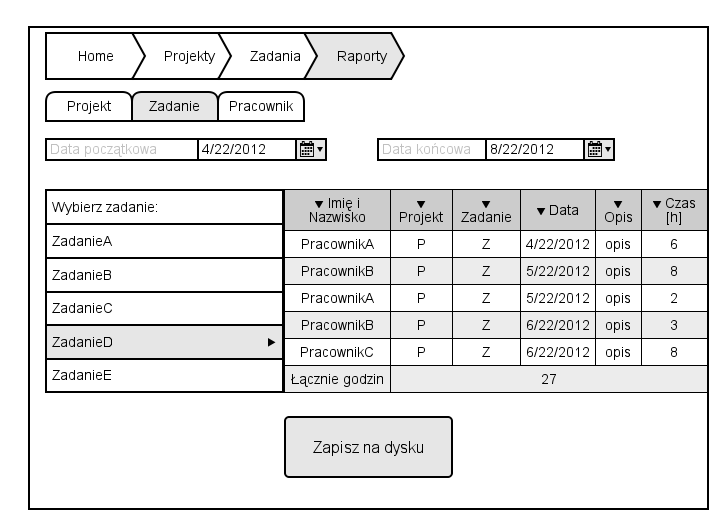
\includegraphics[scale=0.7]{diagramy/intefejsy/Generowanie_raportu_dla_zadania.png}
    \caption{Generowanie raportu dla zadania}
    \label{fig:usecase}
\end{figure}

\subsection{Ekran strony głównej}
\begin{figure}[H]
    \centering
    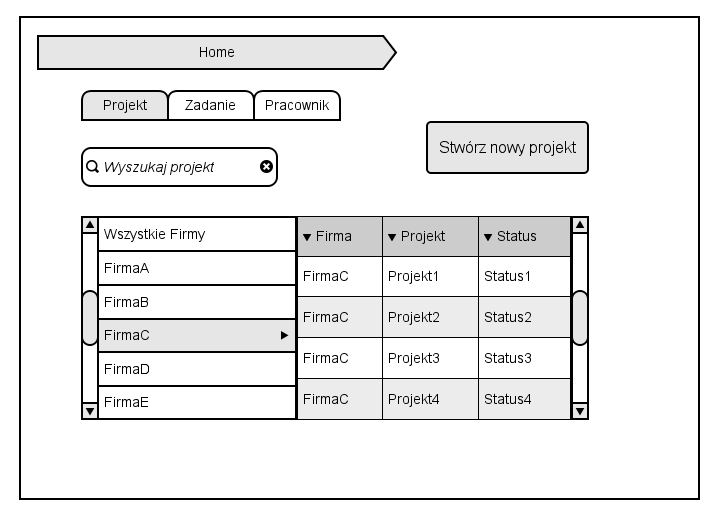
\includegraphics[scale=0.7]{diagramy/intefejsy/Home.png}
    \caption{Strona główna}
    \label{fig:usecase}
\end{figure}

\subsection{Ekran logowania czasu pracy}
\begin{figure}[H]
    \centering
    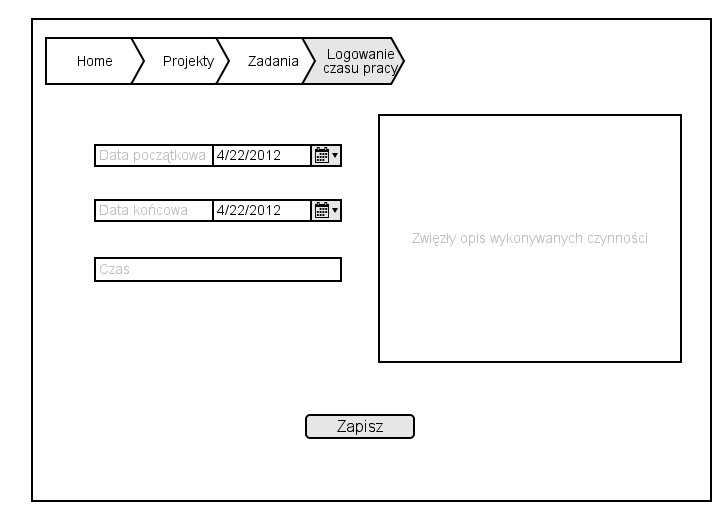
\includegraphics[scale=0.7]{diagramy/intefejsy/Logowanie_czasu_pracy.png}
    \caption{Logowanie czasu pracy}
    \label{fig:usecase}
\end{figure}

\subsection{Ekran edycji projektu}
\begin{figure}[H]
    \centering
    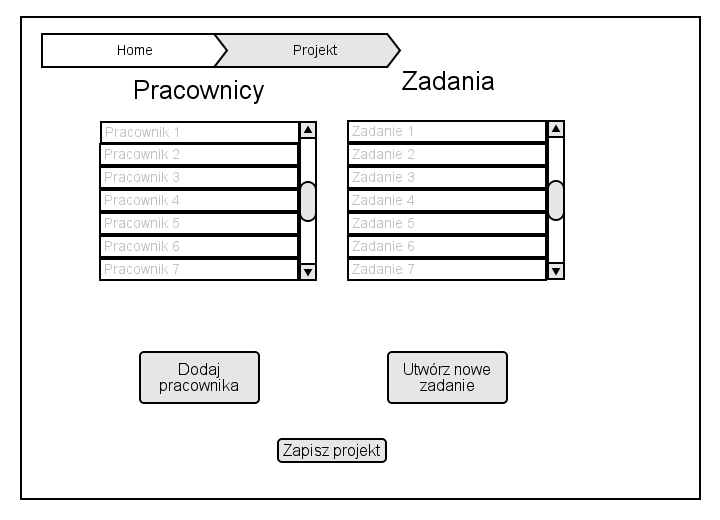
\includegraphics[scale=0.7]{diagramy/intefejsy/Projekt.png}
    \caption{Edycja projektu}
    \label{fig:usecase}
\end{figure}

\subsection{Ekran edycji zespołu projektu}
\begin{figure}[H]
    \centering
    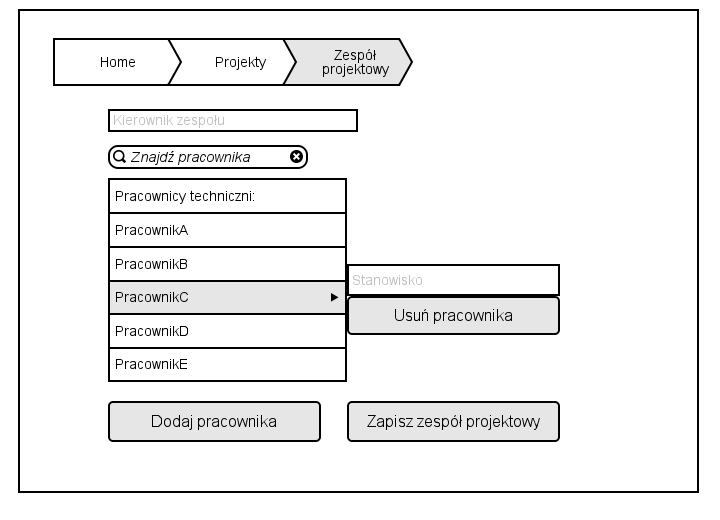
\includegraphics[scale=0.7]{diagramy/intefejsy/Modyfikacja_zespolu_projektowego.png}
    \caption{Modyfikacja zespolu projektowego}
    \label{fig:usecase}
\end{figure}

\subsection{Ekran tworzenia projektu}
\begin{figure}[H]
    \centering
    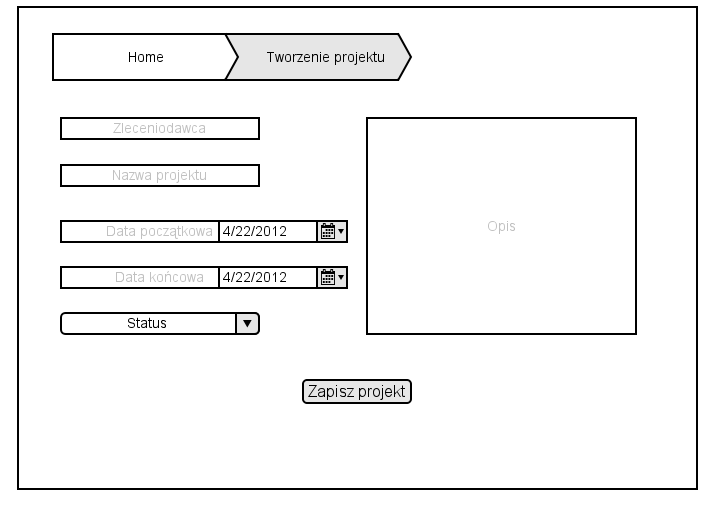
\includegraphics[scale=0.7]{diagramy/intefejsy/Tworzenie_projektu.png}
    \caption{Tworzenie projektu}
    \label{fig:usecase}
\end{figure}

\subsection{Ekran tworzenia zadania}
\begin{figure}[H]
    \centering
    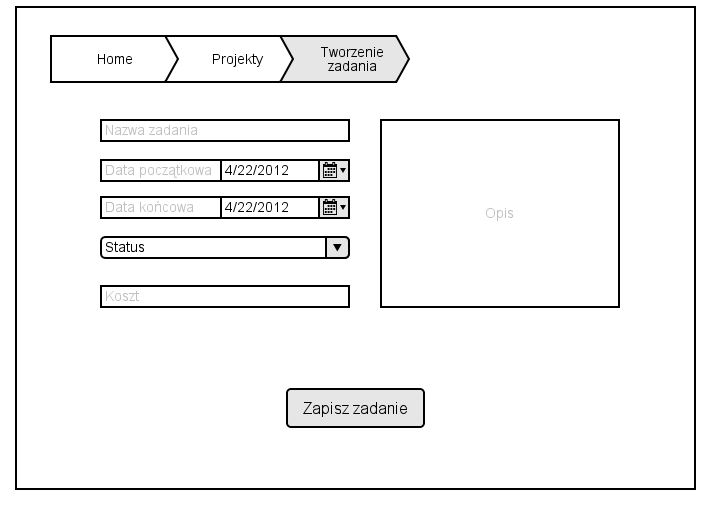
\includegraphics[scale=0.7]{diagramy/intefejsy/Tworzenie_zadania.png}
    \caption{Tworzenie zadania}
    \label{fig:usecase}
\end{figure}

\subsection{Ekran składania wniosku urlopowego}
\begin{figure}[H]
    \centering
    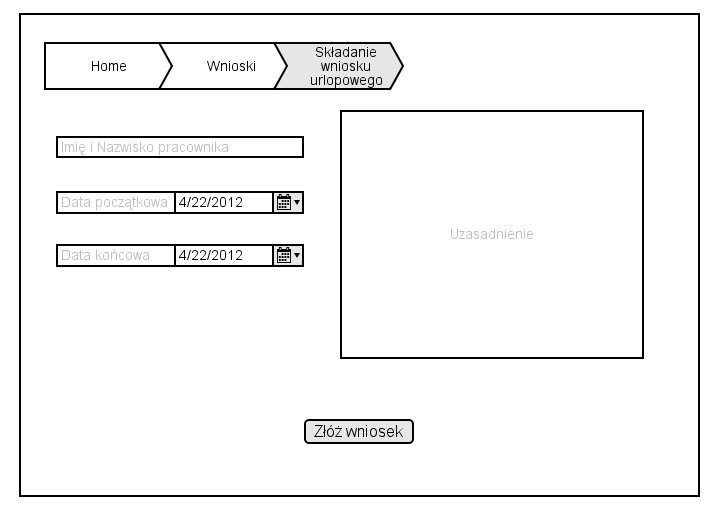
\includegraphics[scale=0.7]{diagramy/intefejsy/Wniosek_urlopowy.png}
    \caption{Wniosek urlopowy}
    \label{fig:usecase}
\end{figure}

\subsection{Ekran przeglądania zadań}
\begin{figure}[H]
    \centering
    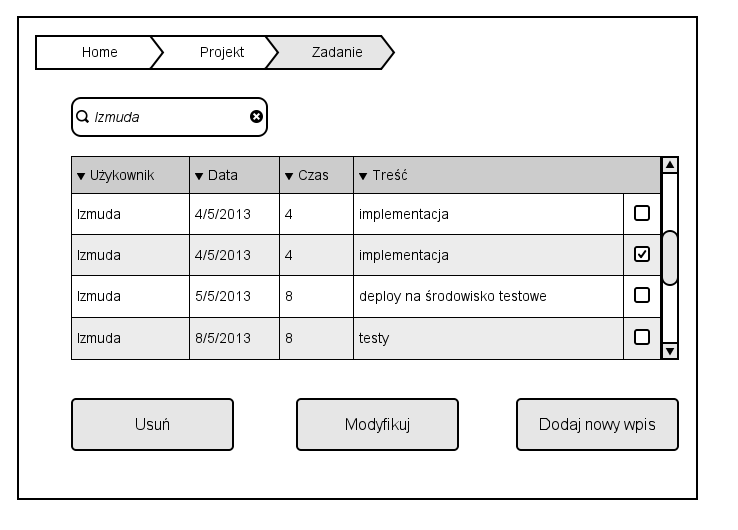
\includegraphics[scale=0.7]{diagramy/intefejsy/Zadanie.png}
    \caption{Zadanie}
    \label{fig:usecase}
\end{figure}
\end{document}


